
\section{Heterogeneous Pretraining Data}
\label{sec:data}

\begin{figure}[t]
  \centering
  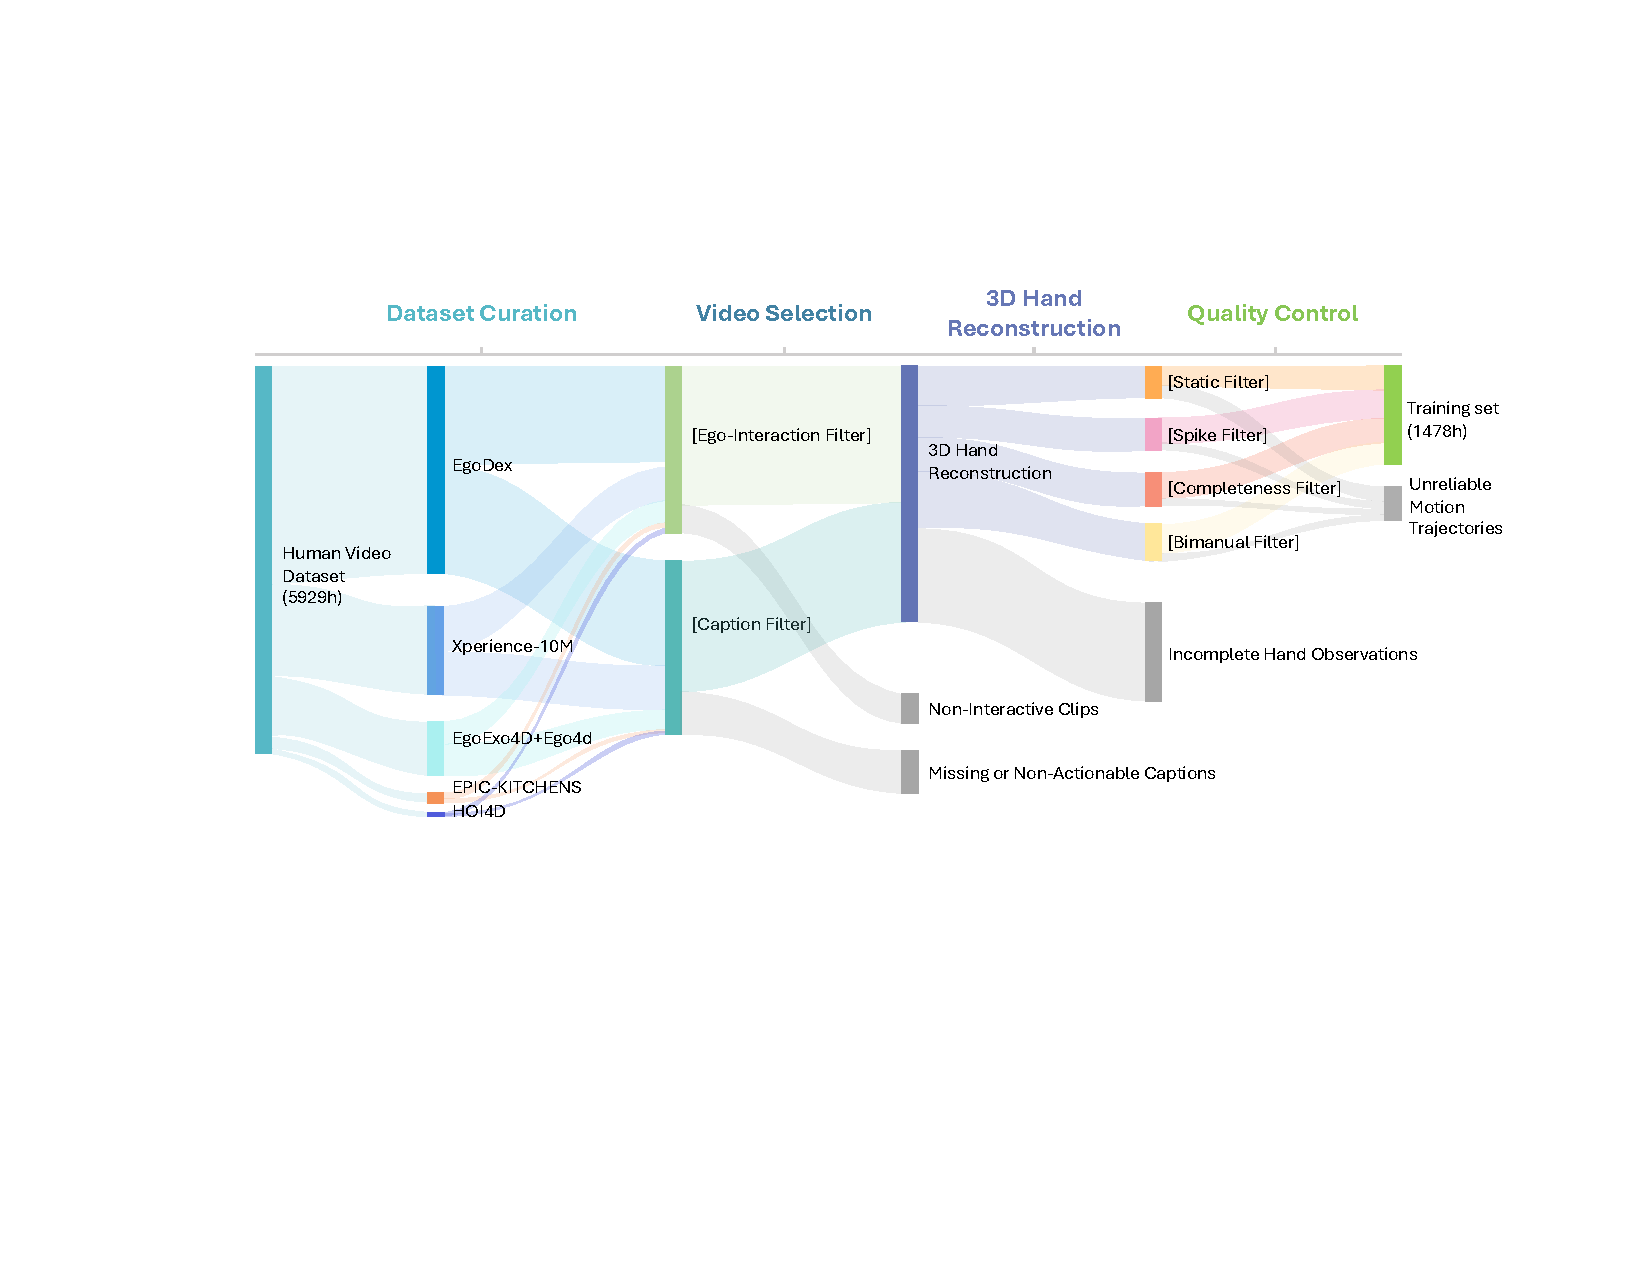
\includegraphics[width=\linewidth]{images/statics.pdf}
  \caption{Overview of the \Ours data processing pipeline for constructing training-ready embodied manipulation data from large-scale egocentric human video. Raw videos pass through video selection, motion reconstruction, and multi-stage quality control, yielding 1,478 hours of pseudo-action-labeled embodied manipulation data that complement the robot and simulation portions of the training pool.}
  \label{fig:statics}
\end{figure}

The \Ours pretraining pool covers the full spectrum of embodied experience, including sensor-logged robot demonstrations across multiple platforms, simulation rollouts, and pseudo-action-labeled egocentric human videos, totaling more than 6.0K hours as shown in Table~\ref{tab:pretraining-data-main}. These sources exhibit significant representation heterogeneity as identified in Section~\ref{sec:introduction}: they differ in spatial coordinate frames, kinematic structures, and control frequencies, and further vary in action-label quality.
Section~\ref{sec:data-sources} catalogs our overall mixed-source datasets, while Section~\ref{sec:human-pipeline} describes the pipeline that converts raw egocentric videos into pseudo-action labels compatible with the unified interface defined in Section~\ref{sec:unified-interface}. Figure~\ref{fig:statics} provides a visual overview of this conversion process.

\subsection{Heterogeneous Data Sources}
\label{sec:data-sources}



\paragraph{Robot demonstrations and simulation.}
The robot portion consists of AgiBot Alpha/Beta demonstrations, Galaxea R1Lite data, AgiBot DigitalWorld simulation rollouts, RoboCasa Tabletop simulation data (24 tasks, 1,000 episodes each, GR1 humanoid robot), and 1,800+ hours of self-collected Galbot demonstrations. These platforms span humanoid (AgiBot G1), single-arm wheeled (Galaxea R1Lite), and mobile bimanual (Galbot) embodiments, with control frequencies ranging from 10 to 30~Hz and end-effector poses logged in different reference frames depending on the platforms. This heterogeneity exposes representation mismatch and motivates the unified interface introduced in Section~\ref{sec:unified-interface}. All sources provide sensor-grounded end-effector action labels, which serve as high-fidelity supervision for the primary action expert in Section~\ref{sec:reliability-aware-objective}.

\paragraph{Human egocentric videos.}
The human-video portion draws from six sources: Ego4D~\cite{grauman2022ego4d}, EgoExo4D~\cite{grauman2024egoexo4d}, EPIC-KITCHENS-100~\cite{damen2018epic}, HOI4D~\cite{liu2022hoi4d}, EgoDex~\cite{hoque2025egodex}, and Xperience-10M~\cite{xperience_10m}. Together, they span diverse kitchens, homes, and workshops, capturing long-tail manipulation behaviors that are difficult to cover via robot teleoperation alone. Since their action labels are inferred from vision-based pipelines rather than physical sensors, we treat them as pseudo-action-labeled supervision and route them through the reliability-aware human objective in Section~\ref{sec:human-auxiliary-loss}.



\begin{table}[h]
\centering
\small
\caption{\Ours pretraining data pool. Hours are computed from dataset metadata as $\text{frames} / (\text{fps} \times 3600)$; Galbot hours are reported from our self-collected collections.}
\label{tab:pretraining-data-main}
\begin{tabular}{lrrrr}
\toprule
Source & Episodes & Frames & Hours & Supervision \\
\midrule
Ego4D & 948,683 & 23,396,157 & 216.6 & Pseudo-action \\
EgoExo4D & 41,414 & 1,110,275 & 10.3 & Pseudo-action \\
EPIC-KITCHENS-100 & 74,788 & 3,486,432 & 32.3 & Pseudo-action \\
HOI4D & 2,966 & 774,275 & 7.2 & Pseudo-action \\
EgoDex & 327,317 & 83,894,075 & 776.8 & Pseudo-action \\
Xperience-10M & 99,027 & 31,370,900 & 435.7 & Pseudo-action \\
\midrule
Human video subtotal & 1,494,195 & 144,032,114 & 1,478.9 & Pseudo-action \\
\midrule
AgiBot Alpha/Beta & 116,013 & 209,284,239 & 1,937.8 & Robot action \\
Galaxea R1Lite & 20,662 & 26,358,560 & 488.1 & Robot action \\
AgiBot DigitalWorld & 47,910 & 24,333,788 & 225.3 & Robot action \\
RoboCasa Tabletop & 24,000 & 6,020,058 & 83.6 & Robot action \\
Galbot self-collected & $\sim$60,000 & $\sim$194M & 1,800+ & Robot action \\
\midrule
Robot subtotal & $\sim$268,585 & $\sim$460M & 4,534.8+ & Robot action \\
\midrule
Total & $\sim$1,762,780 & $\sim$604M & 6,013.7+ & Mixed \\
\bottomrule
\end{tabular}
\end{table}
% \FloatBarrier



\subsection{Egocentric Video-to-Action Conversion}
\label{sec:human-pipeline}


\begin{figure}[htbp]
  \centering
  
\includegraphics[width=\linewidth]{images/data_pipeline.pdf}
  \caption{Pipeline for converting raw egocentric videos into camera-space pseudo-actions. The pipeline consists of five stages: (1)~dataset curation;
  (2)~video selection using ego-interaction and image captioning-based filters;
  (3)~3D hand reconstruction, including 2D tracking, local pose estimation, and trajectory optimization;
  (4)~action parameterization using robot action conventions and human end-effector equivalents; and
  (5)~quality control through multiple filtering.}
  \label{fig:data-pipeline}
\end{figure}

Generating pseudo-labeled actions compatible with robotic data from large-scale video datasets requires bridging two major challenges: the \textit{structural discrepancy}, since 2D video carries no metric 3D hand trajectories, and the \textit{behavioral discrepancy}, since not every clip contains a clean manipulation primitive worth supervising on. We address both with a five-stage pipeline (Figure~\ref{fig:data-pipeline})
that includes clip-level filtering, geometric recovery, action formatting, and fidelity-based quality control. Running this pipeline over six egocentric video datasets, we produce $1{,}478$ hours of pseudo-action-labeled clips that share the same camera-space action format as robot data and enter the unified action space of Section~\ref{sec:unified-interface}. All quantitative
thresholds are collected in Table~\ref{tab:egocentric-pipeline-hparams}. We describe each stage in detail below.

\paragraph{Stage~1: Dataset curation.}
We begin with publicly available human video collections and select sources that satisfy three criteria: an egocentric viewpoint, diverse real-world interaction scenes, and high-quality action-centric captions. This process yields the six datasets listed in
Table~\ref{tab:pretraining-data-main}, which forms our human video pool. We then standardize all sources into a unified storage format with consistent metadata fields, including clip identifiers, frame indices, camera intrinsics (when available), narrations, and licensing
information. For sources that provide only video-level annotations, we split videos into clips. We discard clips that are shorter than 4 seconds or longer than 30 seconds, as they are unlikely to contain complete manipulation primitives at the downstream temporal granularity.

\paragraph{Stage~2: Video selection.}
The previous stage produces a large pool of egocentric videos that vary substantially in interaction quality and manipulation relevance. Before applying computationally intensive geometric reconstruction, we adopt an
\emph{ego-interaction filter} to remove clips that are unlikely to provide useful action supervision. The filter targets videos with limited human-object interaction and employs several lightweight cues to identify such cases. Among them, strong face detections serve as an effective signal of non-egocentric or observer-centric viewpoints, which rarely contain usable manipulation trajectories. We therefore discard clips whose maximum face-detection confidence exceeds a predefined threshold. 
A subsequent \emph{image captioning-based filter} retains only clips whose narrations contain at least one manipulation verb and one manipulable object noun, further enriching the dataset with object-centric interaction behaviors.

\paragraph{Stage~3: 3D hand reconstruction.}
Hand reconstruction is performed in three sub-stages: 2D tracking, local pose estimation, and global trajectory optimization. We first apply a SAM3-based~\cite{sam3} tracker to obtain temporally consistent hand bounding boxes and segmentation masks throughout each clip, and discard detections with keypoint confidence below $\tau_{\mathrm{kp}}$ or track length below $\ell_{\min}$ frames. We then feed the retained hand crops into HaMeR~\cite{pavlakos2024reconstructing}, which reconstructs MANO shape and pose parameters $\{\beta, \theta_t, \mathbf{t}^{\mathrm{local}}_t\}_{t=1}^{T}$ for each frame in hand-related clips. Since per-frame reconstruction suffers from depth ambiguity, occlusions, and temporal jitter, we further perform a two-stage global trajectory optimization inspired by~\cite{dyn}, where the first stage ($N_{\mathrm{root}}$ iterations) estimates globally consistent root translation and orientation, and the second stage ($N_{\mathrm{smooth}}$ L-BFGS iterations) jointly minimizes reprojection error and a temporal smoothness regularizer:
\begin{equation}
\mathcal{L}_{\mathrm{smooth}}
=
\mathcal{L}_{\mathrm{reproj}}
+
\lambda_{\mathrm{tv}}
\sum_t
\left\|
\mathbf{t}^{\mathrm{global}}_{t+1}
-
2\mathbf{t}^{\mathrm{global}}_{t}
+
\mathbf{t}^{\mathrm{global}}_{t-1}
\right\|_2^2 ,
\end{equation}
where $\mathcal{L}_{\mathrm{reproj}}$ denotes the 2D keypoint reprojection loss, $\mathbf{t}^{\mathrm{global}}_t$ is the optimized global hand root translation at frame $t$, and $\lambda_{\mathrm{tv}}$ controls the strength of temporal smoothness regularization. Both optimization stages leverage per-frame camera poses $(\mathbf{R}_t^{\mathrm{cam}}, \mathbf{t}_t^{\mathrm{cam}})$ estimated by VIPE~\cite{vipe}, enabling conversion of local reconstructions into temporally coherent 3D trajectories in a shared world coordinate frame. The optimized global trajectory is used only for temporal consistency; the final pseudo-action labels are transformed back into the corresponding head-camera frame before training.

\paragraph{Stage~4: Action parameterization.}
The parameterization itself (wrist origin, palm-plane orientation,
thumb-to-palm gripper proxy) is defined in
Section~\ref{sec:camera-space-action}. Here we explain two implementation
details. \emph{Storage layout.} On disk, each per-hand action is stored as
a 16-dimensional bimanual vector: $3$ position $+ 3$ XYZ Euler $+ 1$
gripper $+ 1$ activity flag, per hand; $8\text{D} \times 2\text{ hands} = 16\text{D}$ total. At training time the Euler angles
are converted to the continuous 6D rotation
representation~\cite{zhou2019continuity}, producing the $22$-dimensional
action vector, defined in Section~\ref{sec:camera-space-action}.
\emph{Gripper normalization.} Thumb-to-palm distances $d_t$ are linearly
normalized to the robot gripper stroke range: 
$[d_{\min}^{\mathrm{grip}}, d_{\max}^{\mathrm{grip}}]
= [0.04, 0.10]\,\mathrm{m}$. Trajectories whose 10th--90th percentile range
satisfies $d_{90} - d_{10} < \tau_{\mathrm{grip}}$ are treated as
degenerate (e.g., closed-fist motion with no grasp transition) and assigned
a constant neutral gripper state.

% \paragraph{Stage~5: Quality control.}
% Four post-processing filters remove corrupted or behaviorally implausible
% human episodes before they enter the mixed pretraining pool. The
% \emph{completeness filter} requires episodes to be free of NaN/Inf values
% and contiguous in their frame indices, and stored quaternions to satisfy
% $|\|q\|-1| \le \tau_{\mathrm{quat}}$. The \emph{static filter} discards
% episodes in which neither hand exhibits per-second motion energy above
% $\tau_{\mathrm{static}}$. The \emph{spike filter} rejects trajectories
% whose inter-frame positional change exceeds $\kappa_{\mathrm{spike}}\sigma$
% of the per-episode velocity distribution on more than
% $\rho_{\mathrm{spike}}$ of frames. The \emph{bimanual filter} flags
% implausible dual-arm behaviors via anomalous inter-hand distance statistics
% or weak temporal correlation between the two hands; concrete values are
% recorded with the released data manifests, as they depend on source-level
% hand-detection density.
\paragraph{Stage~5: Quality control.}
This stage removes corrupted or behaviorally implausible human episodes before they are collected into the mixed-source pretraining datasets. Here we apply four post-processing filters. 
\emph{Completeness filter.} We require each
episode to be free of NaN/Inf values, contain contiguous frame indices, and satisfy quaternion normalization constraints: $|\|q\|-1| \le \tau_{\mathrm{quat}}$. \emph{Static filter.} We discard episodes when neither hand exhibits per-second motion energy above $\tau_{\mathrm{static}}$, indicating little or no meaningful interaction. 
\emph{Spike filter.} We reject trajectories if inter-frame positional changes exceed $\kappa_{\mathrm{spike}}\sigma$ of the per-episode velocity distribution on more than $\rho_{\mathrm{spike}}$ of frames, which typically indicates tracking failures or reconstruction artifacts.
\emph{Bimanual filter.} We remove episodes with implausible dual-arm behaviors based on anomalous inter-hand distance statistics or weak temporal correlation between the two hands. We record the corresponding thresholds in the released data manifests since they depend on source-level hand-detection density.

\begin{table}[!t]
\centering
\small
\caption{Egocentric video pipeline hyperparameters used in Stages~1--5. Values are shared across the six human-video sources
unless noted otherwise.}
\label{tab:egocentric-pipeline-hparams}
\renewcommand{\arraystretch}{1.1}
\begin{tabular}{lll}
\toprule
\textbf{Stage} & \textbf{Hyperparameter} & \textbf{Value} \\
\midrule
\multirow[t]{2}{*}{Stage 1: Curation}
  & Min clip duration                               & 4~s \\
  & Max clip duration                               & 30~s \\
\midrule
\multirow[t]{2}{*}{Stage 2: Selection}
  & Face-detection threshold                        & 0.5 \\
  & Caption verb/noun requirement                   & both present \\
\midrule
\multirow[t]{5}{*}{Stage 3: Reconstruction}
  & Keypoint confidence $\tau_{\mathrm{kp}}$        & 0.4 \\
  & Min track length $\ell_{\min}$                  & 15 frames \\
  & Root-fitting iterations $N_{\mathrm{root}}$     & 30 \\
  & Smooth-fitting iterations $N_{\mathrm{smooth}}$ & 200 \\
  & Smoothness weight $\lambda_{\mathrm{tv}}$       & 1.0 \\
\midrule
\multirow[t]{3}{*}{Stage 4: Parameterization}
  & Gripper stroke range $[d_{\min}^{\mathrm{grip}}, d_{\max}^{\mathrm{grip}}]$ & $[0.04, 0.10]\,\mathrm{m}$ \\
  & Gripper-degeneracy threshold $\tau_{\mathrm{grip}}$ & 1.5~cm \\
  & On-disk action dim / training action dim        & 16-D / 22-D \\
\midrule
\multirow[t]{4}{*}{Stage 5: Filtering}
  & Quaternion tolerance $\tau_{\mathrm{quat}}$     & $10^{-3}$ \\
  & Static motion energy $\tau_{\mathrm{static}}$   & source-specific \\
  & Spike $\sigma$-multiplier $\kappa_{\mathrm{spike}}$ & 3 \\
  & Spike frame fraction $\rho_{\mathrm{spike}}$    & 5\% \\
\bottomrule
\end{tabular}
\end{table}

